% 画幅切换：aspectratio=43（4:3）↔ aspectratio=169（16:9，当前）
\documentclass[10pt,aspectratio=169,hyperref={colorlinks,citecolor=peking_blue,urlcolor=peking_blue,linkcolor=}]{beamer}
\usepackage{PekingU}
\usefonttheme{serif}
\usepackage{lipsum}
% 中文支持：需用 XeLaTeX 编译（latexmk -xelatex main.tex）
% 中文衬线宋体：macOS 用 Songti SC；其他环境（Linux/Overleaf 等）自动回退到
% TeX Live 自带的 FandolSong（按文件名经 kpathsea 加载，不依赖系统字体）
\usepackage[fontset=none, scheme=plain]{ctex}
\IfFontExistsTF{Songti SC}{%
  \setCJKmainfont{Songti SC}[AutoFakeSlant=0.2]%
  \setCJKsansfont{Songti SC}[AutoFakeSlant=0.2]%
  \setCJKmonofont{Songti SC}%
}{%
  \setCJKmainfont{FandolSong-Regular}[Extension=.otf,BoldFont=FandolSong-Bold,AutoFakeSlant=0.2]%
  \setCJKsansfont{FandolSong-Regular}[Extension=.otf,BoldFont=FandolSong-Bold,AutoFakeSlant=0.2]%
  \setCJKmonofont{FandolFang-Regular}[Extension=.otf,BoldFont=FandolFang-Regular]%
}
\usepackage{hyperref}
\setmainfont{XCharter} % Nicer fonts — the charter package is ignored under XeLaTeX, so use fontspec instead
% 等宽字体：优先 Maple Mono NF（静态字族，真实粗/斜体），其次可变版，未安装则回退默认
\IfFontExistsTF{Maple Mono NF}{%
  \setmonofont{Maple Mono NF}[Scale=MatchLowercase,Ligatures=TeX]%
}{%
  \IfFontExistsTF{Maple Mono}{%
    \setmonofont{Maple Mono}[Scale=MatchLowercase,Ligatures=TeX]%
  }{}%
}
% other packages
\usepackage{latexsym,amsmath,xcolor,multicol,booktabs,calligra}
\usepackage{amssymb}
\usepackage{graphicx}
\usepackage{tikz}
\usepackage{bm}
\usepackage{natbib}
\usepackage{wrapfig}
\usepackage{amsfonts} 
\usepackage{ragged2e}
\usepackage{parskip}

\apptocmd{\frame}{}{\justifying}{} % Allow optional arguments after frame.

% 引用整体着色为 peking_blue（与 definition block 标题蓝一致）：
% natbib 的 \citep/\citet 括号不在 hyperref 链接内，仅靠 citecolor 只能染色链接部分，
% 此处将整个引用（含括号）包进颜色组。
\makeatletter
\NewCommandCopy{\pku@citep@orig}{\citep}
\NewCommandCopy{\pku@citet@orig}{\citet}
\RenewDocumentCommand{\citep}{o o m}{%
  \begingroup\color{peking_blue}%
  \IfNoValueTF{#1}{\pku@citep@orig{#3}}%
    {\IfNoValueTF{#2}{\pku@citep@orig[][#1]{#3}}%
      {\pku@citep@orig[#1][#2]{#3}}}%
  \endgroup}
\RenewDocumentCommand{\citet}{o o m}{%
  \begingroup\color{peking_blue}%
  \IfNoValueTF{#1}{\pku@citet@orig{#3}}%
    {\IfNoValueTF{#2}{\pku@citet@orig[][#1]{#3}}%
      {\pku@citet@orig[#1][#2]{#3}}}%
  \endgroup}
\makeatother

\newcommand{\theHalgorithm}{\arabic{algorithm}}
\theoremstyle{plain}
\newtheorem{axiom}{Axiom}
\newtheorem{claim}[axiom]{Claim}
\newtheorem{assumption}{Assumption}
\newtheorem{remark}{Remark}
\newtheorem{proposition}{Proposition}
\setbeamertemplate{theorems}[numbered] 


% change for your title page information
\author[Yiran Rex Ma 马义然]{Yiran Rex Ma \; 马义然\\{\small\href{mailto:yiranrexma@outlook.com}{\texttt{yiranrexma@outlook.com}}}}
\title[Minimalist PKU Beamer 2026]{Minimalist PKU Beamer 2026}
\subtitle{A lightweight PKU-style Beamer template with Chinese support}
\institute{Institute of Linguistics and Applied Linguistics, Peking University}
\date{2026/09/11}

% 右上角校徽（与标题条同高、严格对齐）由 PekingU.sty 中的 frametitle 模板绘制
% official colors match with the PKU red
\def\cmd#1{\texttt{\color{red}\footnotesize $\backslash$#1}}
\def\env#1{\texttt{\color{blue}\footnotesize #1}}
\definecolor{deepblue}{rgb}{0,0,0.5}
\definecolor{deepred}{rgb}{0.6,0,0}
\definecolor{deepgreen}{rgb}{0,0.5,0}
\definecolor{halfgray}{gray}{0.55}

\begin{document}
{
\setbeamertemplate{logo}{}
\begin{frame}
    \titlepage
    \begin{figure}[htpb]
        \begin{center}
            
\includegraphics[width=0.275\linewidth]{Figures/PKU-emblem-names.png}
        \end{center}
    \end{figure}
\end{frame}
}

\section{Introduction}

% 中文排版示例（可删除）：中英文混排、粗体、斜体
\begin{frame}{中文支持示例}
北京大学（Peking University）创建于 1898 年，初名\textbf{京师大学堂}。

\begin{itemize}
    \item 中文正文使用衬线\textbf{宋体}（Songti SC），与英文 XCharter 衬线字体搭配
    \item 等宽字体为 \texttt{Maple Mono}：\texttt{0O Il 1l \{[(=+])\}}
    \item {\itshape 斜体中文通过伪斜体自动生成，}数学公式不受影响：$\int_0^\infty e^{-x^2}\,\mathrm{d}x = \frac{\sqrt{\pi}}{2}$
    \item 标点符号使用全角样式：“引号”、‘单引号’、破折号——省略号……
\end{itemize}

\begin{theorem}[中文定理示例]
    若函数 $f(x)$ 在闭区间 $[a,b]$ 上连续，则 $f(x)$ 在 $[a,b]$ 上必有最大值与最小值。
\end{theorem}
\end{frame}

\begin{frame}{How to cite in your introduction?}
\lipsum[1][1-3]

\begin{enumerate}
    \item \lipsum[1][1-2] \citep{langley00}
    \item \citet {mitchell80} \lipsum[1][3-4] 
    \item \lipsum[1][5-6] \citep{kearns89}
\end{enumerate}

important contents are \textcolor{peking}{\bf bold red} \citep{MachineLearningI}. 
\lipsum[1][1-4]
\end{frame}

\begin{frame}{Wrapping text around figures}
    \begin{wrapfigure}{r}{0.4\textwidth}
      \begin{center}
        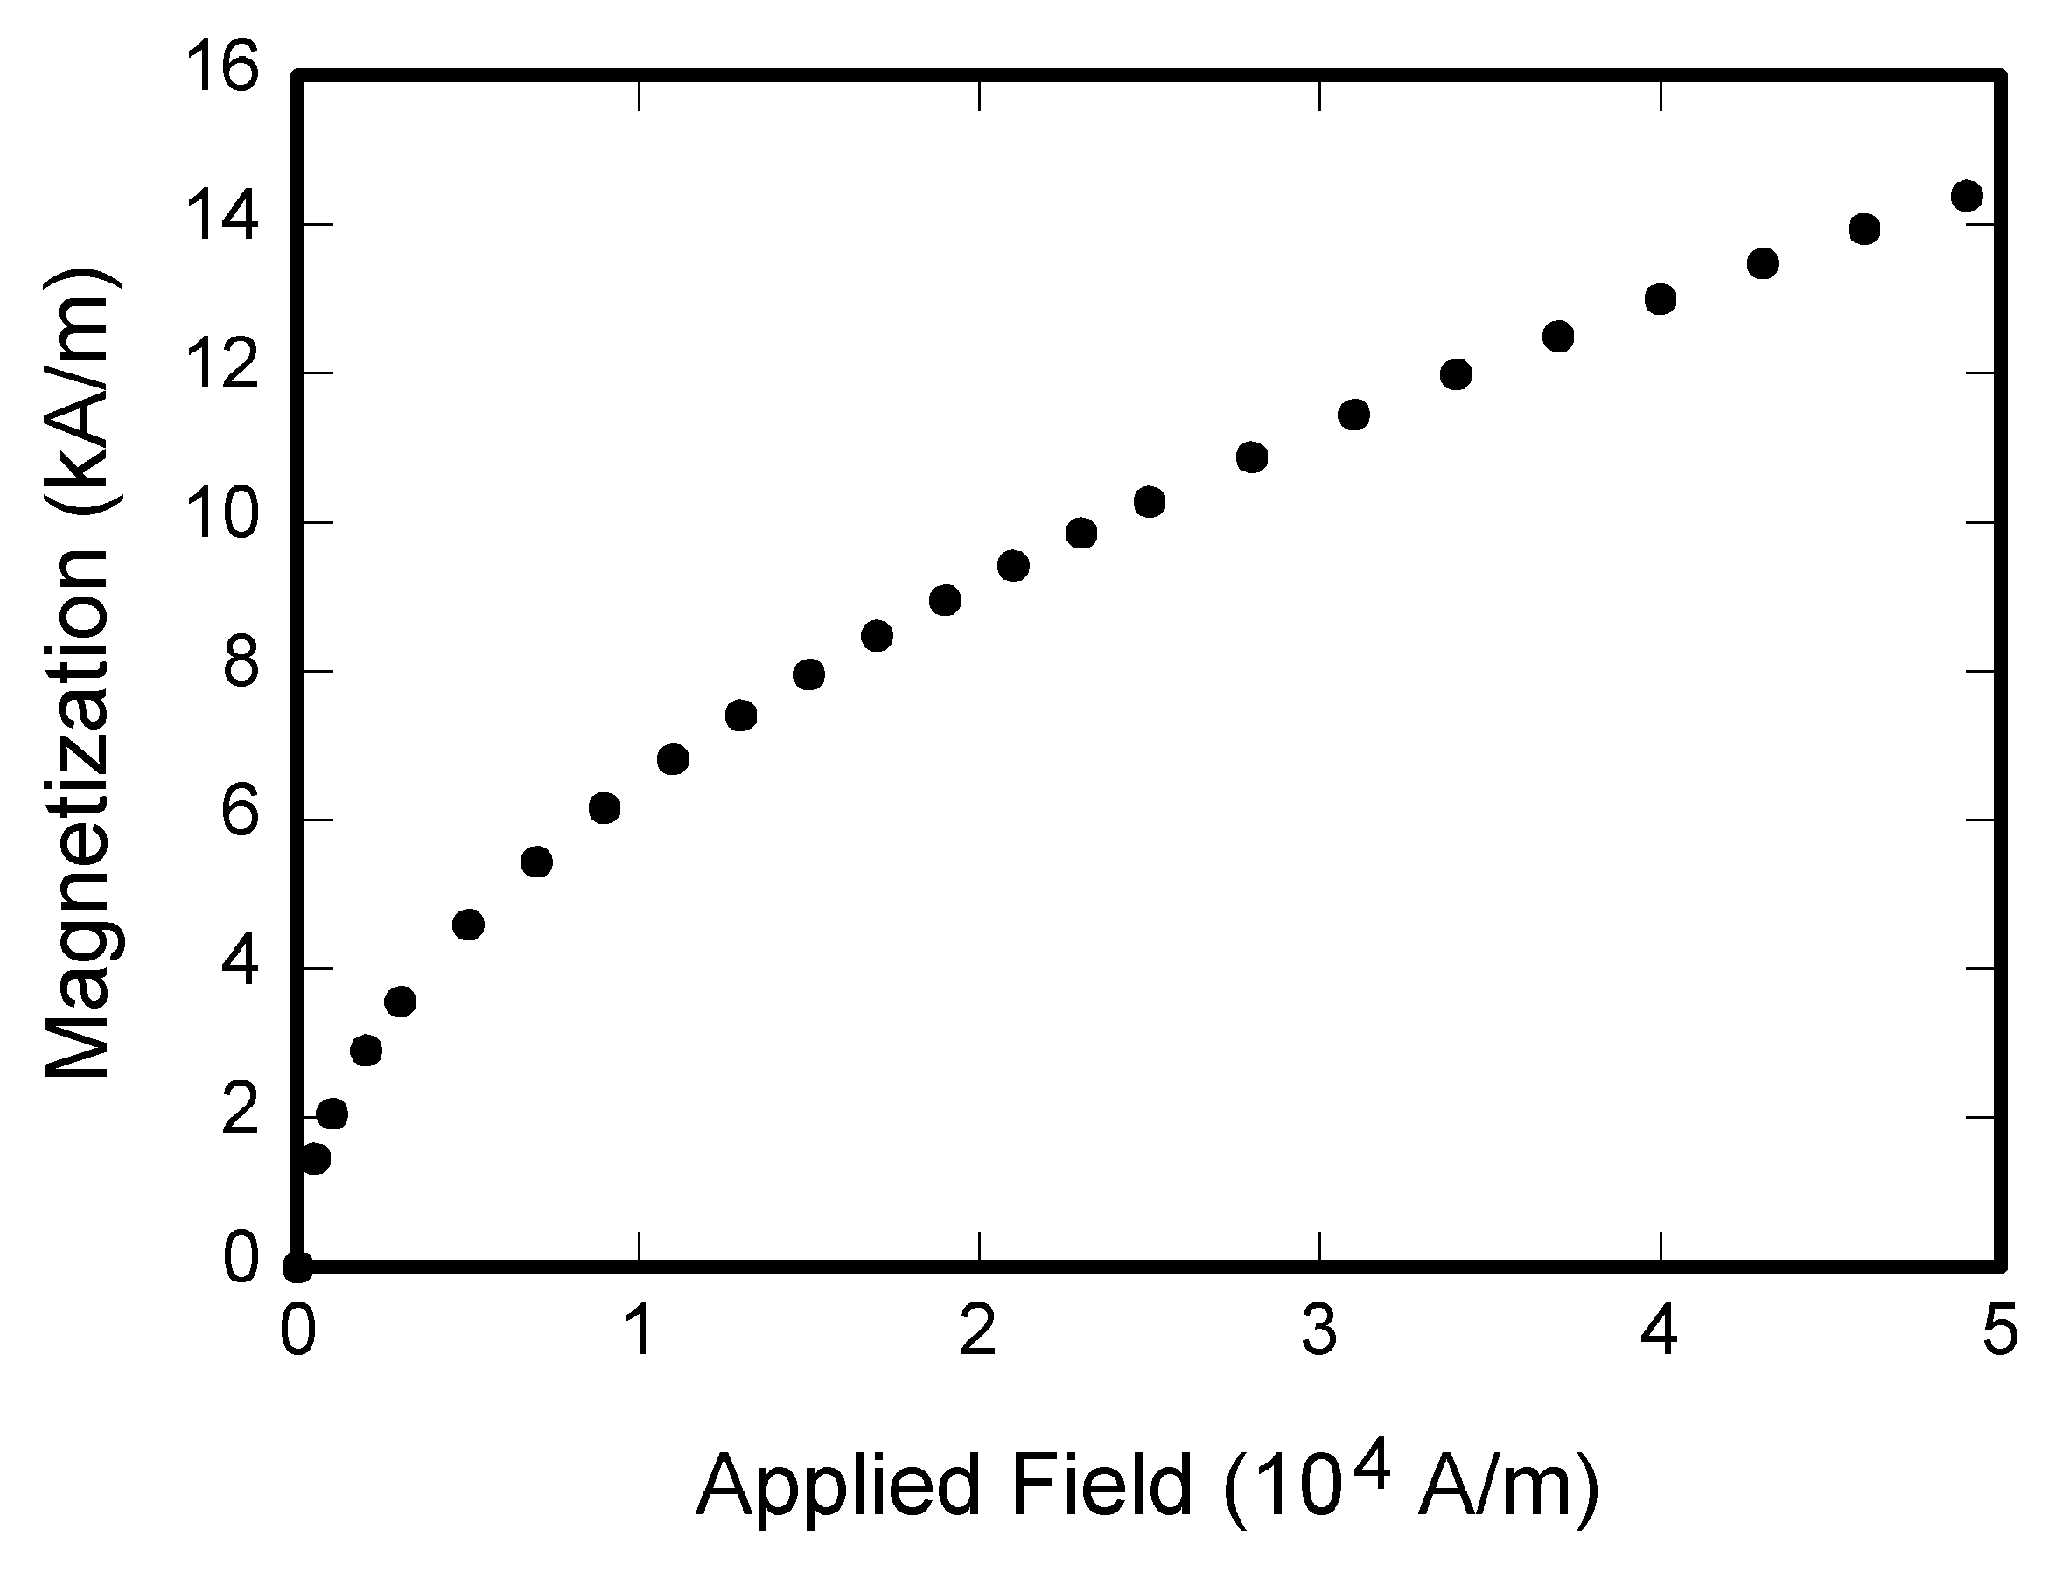
\includegraphics[width=0.4\textwidth]{Figures/fig1.png}
      \end{center}
      \caption{\lipsum[1][1-1]}
    \end{wrapfigure}
    
    \lipsum[1][1-4]

    \lipsum[1][5-10]

    \lipsum[2][1-3]
\end{frame}

\begin{frame}{Mathematical expressions}
    \lipsum[3][1-5]

    \lipsum[4][1-3]
    \begin{equation}\label{eq:1}
        \bm Y = \bm G \bm X + \bm E,
    \end{equation}
    where 
    \begin{itemize}
        \item $\bm G\in \mathbb{R}^{N\times SO}$ is a known gain matrix, 
        \item $\bm E$ is the IID Gaussian error with $e_{ij}\sim\mathcal{N}(0,\sigma^2)$, 
        \item \lipsum[2][1]
    \end{itemize}
\end{frame}

\section{Motivations}

\begin{frame}{Add block in text}
\lipsum[3][1-3]

\lipsum[3][1-2]

\lipsum[3][1-4]

\begin{block}{What is Few-Shot Learning?}
    \lipsum[3][1-4]
\end{block}
\end{frame}

\section{Methods}

\begin{frame}{Definition, Proposition and Theorem}

\begin{definition}[some explanations]
\lipsum[3][1-4]
\end{definition}

\begin{proposition}\label{prop:1}
\lipsum[3][5-8]
\end{proposition}

\begin{theorem}\label{theorem:generalization bound}
\lipsum[3][9-12]
\end{theorem}
    
\end{frame}

\section{Simulation}

\begin{frame}{Tables}
    \begin{table}
        \caption{Units for Magnetic Properties}
        \label{table}
        \setlength{\parskip}{0pt}% caption 与表头之间不插入段间距
        \footnotesize
        \setlength{\tabcolsep}{3pt}
        \begin{tabular}{p{40pt}p{100pt}p{140pt}}
        \toprule
        {\bfseries Symbol}&
        {\bfseries Quantity}&
        {\bfseries Conversion from Gaussian and \par CGS EMU to SI $^{\mathrm{a}}$} \\
        \midrule
        $\Phi $& 
        magnetic flux& 
        1 Mx $\to  10^{-8}$ Wb $= 10^{-8}$ V$\cdot $s \\
        $B$& 
        magnetic flux density, \par magnetic induction& 
        1 G $\to  10^{-4}$ T $= 10^{-4}$ Wb/m$^{2}$ \\
        $H$& 
        magnetic field strength& 
        1 Oe $\to  10^{3}/(4\pi )$ A/m \\
        $m$& 
        magnetic moment& 
        1 erg/G $=$ 1 emu \par $\to 10^{-3}$ A$\cdot $m$^{2} = 10^{-3}$ J/T \\
        $M$& 
        magnetization& 
        1 erg/(G$\cdot $cm$^{3}) =$ 1 emu/cm$^{3}$ \par $\to 10^{3}$ A/m \\
        4$\pi M$& 
        magnetization& 
        1 G $\to  10^{3}/(4\pi )$ A/m \\
        $\sigma $& 
        specific magnetization& 
        1 erg/(G$\cdot $g) $=$ 1 emu/g $\to $ 1 A$\cdot $m$^{2}$/kg \\
        \bottomrule
        \multicolumn{3}{p{280pt}}{Vertical lines are optional in tables. Statements that serve as captions for 
        the entire table do not need footnote letters. }
        \end{tabular}
        \label{tab1}
    \end{table}
\end{frame}


\begin{frame}{References}%[allowframebreaks] if too many references
    \renewcommand*{\bibfont}{\footnotesize}
    \bibliography{ref}
    \bibliographystyle{apalike}
    % \tiny\bibliographystyle{alpha}
\end{frame}

\begin{frame}
    \begin{center}
        {\Huge\calligra Thanks!}
    \end{center}
\end{frame}

\end{document}